% Figure 0: QA Geometry Overview (TikZ)
\documentclass[tikz,border=4pt]{standalone}
\usepackage{amsmath,amssymb}
\usetikzlibrary{arrows.meta,positioning,decorations.pathreplacing}

\begin{document}
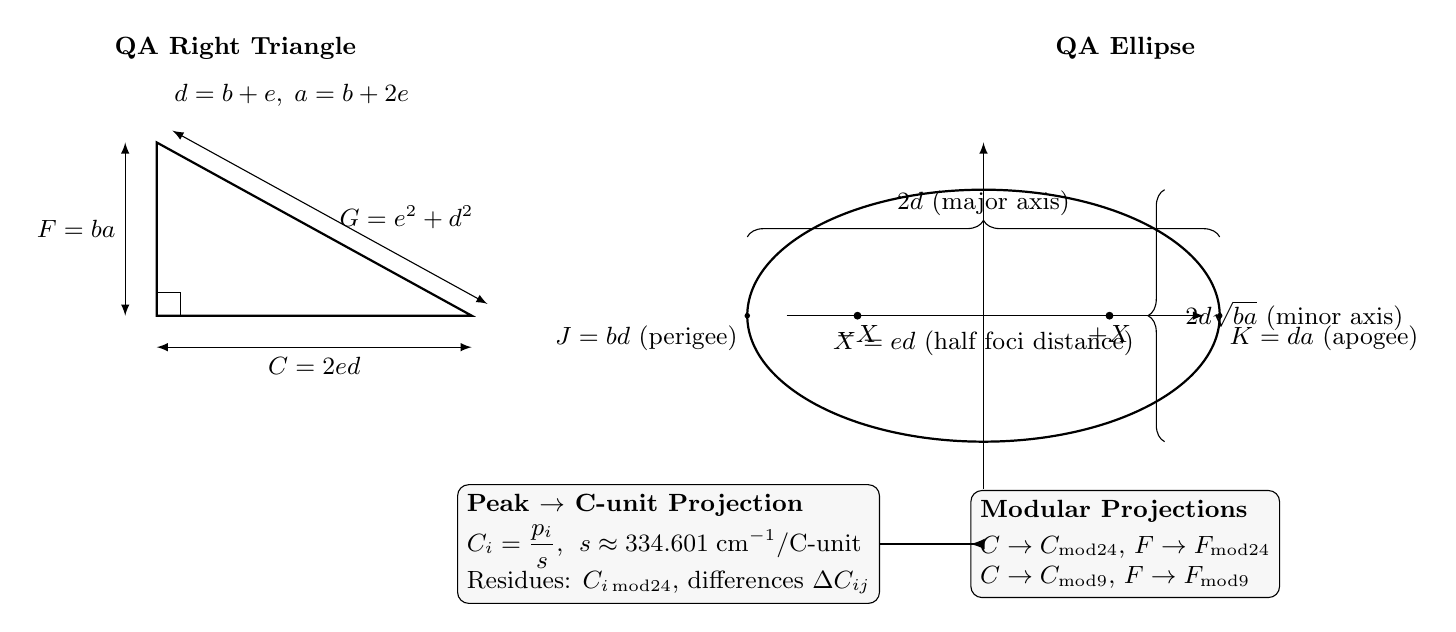
\begin{tikzpicture}[>=latex, font=\small]

%--------------------
% Left: QA Right Triangle (C,F,G)
%--------------------
\node[align=left] (triTitle) at (-7.5,3.4) {\textbf{QA Right Triangle}};

% Triangle points
\coordinate (A) at (-8.5,0.0);   % origin of triangle
\coordinate (B) at (-4.5,0.0);   % along C
\coordinate (Cpt) at (-8.5,2.2); % along F

% Draw triangle
\draw[thick] (A) -- (B) -- (Cpt) -- cycle;

% Right angle marker
\draw (-8.5,0) ++(0.3,0) -- ++(0,0.3) -- ++(-0.3,0);

% Labels on sides
\draw[<->] (-8.5,-0.4) -- node[below] {$C=2ed$} (-4.5,-0.4);
\draw[<->] (-8.9,0) -- node[left] {$F=ba$} (-8.9,2.2);
\draw[<->] (-4.3,0.15) -- node[right] {$G=e^2+d^2$} (-8.3,2.35);

% Equations node
\node[align=left, anchor=west] at (-8.4,2.8) {$d=b+e,\; a=b+2e$};

%--------------------
% Right: QA Ellipse (J,X,K), axes and braces
%--------------------
\node[align=left] (ellTitle) at (3.8,3.4) {\textbf{QA Ellipse}};

% Ellipse parameters (drawn schematically)
\def\a{3.0} % semi-major ~ d (schematic)
\def\b{1.6} % semi-minor ~ d*sqrt{ba} (schematic)

% Axes
\draw[->] (-0.5,0) -- (4.8,0) node[right]{};
\draw[->] (2.0,-2.2) -- (2.0,2.2) node[above]{};

% Ellipse centered at (2,0)
\draw[thick] (2,0) ellipse [x radius=\a, y radius=\b];

% Foci conceptually at +/- X along major axis (schematic)
\filldraw (2-1.6,0) circle (1.2pt) node[below] {$-X$};
\filldraw (2+1.6,0) circle (1.2pt) node[below] {$+X$};
\node[below=2pt] at (2,0) {$X=ed$ (half foci distance)};

% Major/minor axes braces
\draw[decorate,decoration={brace,amplitude=6pt}] (2-\a,1.0) -- node[above=4pt] {$2d$ (major axis)} (2+\a,1.0);
\draw[decorate,decoration={brace,amplitude=6pt}] (4.3,0-\b) -- node[right=4pt] {$2d\sqrt{ba}$ (minor axis)} (4.3,0+\b);

% Perigee/Apogee labels (schematic points)
\fill (2-\a,0) circle (1.0pt) node[below left] {$J=bd$ (perigee)};
\fill (2+\a,0) circle (1.0pt) node[below right] {$K=da$ (apogee)};

%--------------------
% Modular projections and peak -> C mapping
%--------------------
\node[draw, align=left, rounded corners, fill=black!3] (mods) at (3.8,-2.9) {
  \textbf{Modular Projections}\\[2pt]
  $C\to C_{\mathrm{mod}24}$, $F\to F_{\mathrm{mod}24}$\\
  $C\to C_{\mathrm{mod}9}$, $F\to F_{\mathrm{mod}9}$
};

\node[draw, align=left, rounded corners, fill=black!3] (peaks) at (-2.0,-2.9) {
  \textbf{Peak $\to$ C-unit Projection}\\[2pt]
  $C_i = \dfrac{p_i}{s}$,\; $s\approx 334.601\;\mathrm{cm}^{-1}$/C-unit\\
  Residues: $C_{i\,\mathrm{mod}24}$, differences $\Delta C_{ij}$
};

\draw[->,thick] (peaks.east) -- +(1.2,0) |- (mods.west);

\end{tikzpicture}
\end{document}

